\documentclass[degree=bachelor,tocarialchapter,language=english]{thuthesis}
% 选项
%   degree=[bachelor|master|doctor|postdoctor], % 必选,学位类型
%   language=[chinese|english], % 可选(默认:chinese),论文的主要语言
%   secret,                % 可选(默认:关闭),是否有密级
%   tocarialchapter,       % 可选(默认:关闭),章目录中使用黑体(这项表示同时打开下面两项)
%   tocarialchapterentry,  % 可选(默认:关闭),单独控制章标题在目录中使用黑体
%   tocarialchapterpage,   % 可选(默认:关闭),单独控制章页码在目录中使用黑体

% 所有其它可能用到的包都统一放到这里了,可以根据自己的实际添加或者删除。
\usepackage{thuthesis}
\usepackage{fmtcount}
\usepackage{tabulary}

% 定义所有的图片文件在 figures 子目录下
\graphicspath{{figures/}}

% 可以在这里修改配置文件中的定义。导言区可以使用中文。
% \def\myname{薛瑞尼}

\newcommand{\engchapter}[1]{
    \renewcommand{\thechapter}{\Numberstring{chapter}}
    \chapter{#1}
    \renewcommand{\thechapter}{\arabic{chapter}}
}

\newcommand{\citebelong}[1]{
    \citeauthor{#1}'s \citeyearpar{#1}
}

\begin{document}

%%% 封面部分
\frontmatter
\thusetup{
  %******************************
  % 注意:
  %   1. 配置里面不要出现空行
  %   2. 不需要的配置信息可以删除
  %******************************
  %
  %=====
  % 秘级
  %=====
  %
  %=========
  % 中文信息
  %=========
  ctitle={中国计算机科学研究生学术论文写作中引用行为的研究},
  cdegree={文学学士},
  cdepartment={外国语言文学系},
  cmajor={英语语言文学},
  cauthor={姚沛然},
  csupervisor={颜奕\hskip0.6cm 副教授},
  % 日期自动使用当前时间,若需指定按如下方式修改:
  % cdate={超新星纪元},
  %
  %=========
  % 英文信息
  %=========
  etitle={Citation Behaviors of Chinese Computer Science Graduate Students in Research Paper Writing},
  % 这块比较复杂,需要分情况讨论:
  % 1. 学术型硕士
  %    edegree:必须为Master of Arts或Master of Science(注意大小写)
  %             “哲学、文学、历史学、法学、教育学、艺术学门类,公共管理学科
  %              填写Master of Arts,其它填写Master of Science”
  %    emajor:“获得一级学科授权的学科填写一级学科名称,其它填写二级学科名称”
  % 2. 专业型硕士
  %    edegree:“填写专业学位英文名称全称”
  %    emajor:“工程硕士填写工程领域,其它专业学位不填写此项”
  % 3. 学术型博士
  %    edegree:Doctor of Philosophy(注意大小写)
  %    emajor:“获得一级学科授权的学科填写一级学科名称,其它填写二级学科名称”
  % 4. 专业型博士
  %    edegree:“填写专业学位英文名称全称”
  %    emajor:不填写此项
  % 日期自动生成,若需指定按如下方式修改:
  % edate={December, 2005},
  %
  % 关键词用“英文逗号”分割
  ckeywords={引用行为, 外语写作, 学术英语教学},
  ekeywords={citation behaviros, L2 writing, EAP pedagogy}
}

% 定义中英文摘要和关键字
\begin{cabstract}
  恰当引用文献是研究生必备的基本学术素养之一。然而,引用文献涉及到多种认知过程、多方面语言知识,因此是一个较难培养的素养。近期的研究表明,通过文本分析研究引用行为可帮助学术英语教师指导学生引用文献、帮助培养学生引用文献这一学术素养;另外,学术英语教师对学生引用文献的指导应因学科而异。因此,为帮助学术英语教师指导中国计算机科学专业研究生恰当引用文献,本研究分析了11个中国的一年级计算机科学专业研究生的研究论文,并以此研究他们的引用行为。研究使用的语料库由10篇研究论文构成,这些论文是所研究的研究生在旨在指导学生写作和发表学术论文的一年级学术英语写作课程的作业。本研究从引用的形式、目的、质量三个角度对语料库进行了分析,并总结了被研究群体引用行为的特点和不足。基于引用行为分析的结果,本研究还讨论了对教师指导学生学术英语写作的启示及未来研究的可能方向。
\end{cabstract}

% 如果习惯关键字跟在摘要文字后面,可以用直接命令来设置,如下:
% \ckeywords{\TeX, \LaTeX, CJK, 模板, 论文}

\begin{eabstract}
  Using citations is one of the basic but vital academic literacies for graduate students to succeed in academic communities. However, this literacy is not easy to develop as it involves multiple cognitive and linguistic processes. Recent studies have shown that text analysis of citation behaviors could help EAP teachers instruct students on using citations, and the instructions should be adapted according to the group of writers. Therefore, we conducted an analysis of the citation behaviors of a group of 11 first-year Chinese computer science graduate students based on their research papers, in order to help teachers instruct this group of writers. The citation quality, forms and functions were analyzed using a corpus composed of 10 research papers written by these students as part of the requirements of a course aimed at assisting first-year graduate students writing and publishing research papers. The analysis has revealed characteristics and deficiencies of the citation use of this group of students.  In light of the findings of this study, implications for the instruction of academic English writing are discussed, as are considerations for future research.
\end{eabstract}

% \ekeywords{\TeX, \LaTeX, CJK, template, thesis}

% 如果使用授权说明扫描页,将可选参数中指定为扫描得到的 PDF 文件名,例如:
% \makecover[scan-auth.pdf]
\makecover

%% 目录
\tableofcontents

%% 符号对照表
\begin{denotation}[3cm]

\item[AAAI] Association for the Advancement of Artificial Intelligence
\item[ACM] Association for Computing Machinery
\item[APA] American Psychological Association
\item[CARS] Creating a Research Space
\item[CS] computer science
\item[EAP] English for academic purposes
\item[GB/T] \textit{guo biao / tuijian} (national recommended standard)
\item[IEEE] Institute of Electrical and Electronics Engineers
\item[L1] first language
\item[L2] second language
\item[TXT]	text under study

\end{denotation}



% % 也可以使用 nomencl 宏包:

% \printnomenclature[3cm]

% \nomenclature{HPC}{高性能计算 (High Performance Computing)}
% \nomenclature{cluster}{集群}
% \nomenclature{Itanium}{安腾}
% \nomenclature{SMP}{对称多处理}
% \nomenclature{API}{应用程序编程接口}
% \nomenclature{PI}{聚酰亚胺}
% \nomenclature{MPI}{聚酰亚胺模型化合物,N-苯基邻苯酰亚胺}
% \nomenclature{PBI}{聚苯并咪唑}
% \nomenclature{MPBI}{聚苯并咪唑模型化合物,N-苯基苯并咪唑}
% \nomenclature{PY}{聚吡咙}
% \nomenclature{PMDA-BDA}{均苯四酸二酐与联苯四胺合成的聚吡咙薄膜}
% \nomenclature{$\Delta G$}{活化自由能 (Activation Free Energy)}
% \nomenclature{$\chi$}{传输系数 (Transmission Coefficient)}
% \nomenclature{$E$}{能量}
% \nomenclature{$m$}{质量}
% \nomenclature{$c$}{光速}
% \nomenclature{$P$}{概率}
% \nomenclature{$T$}{时间}
% \nomenclature{$v$}{速度}

\mainmatter

%%% 正文部分

\engchapter{Introduction}
\label{chap:intro}

\section{Background}
Using citations is one of the basic but essential literacies in academic writing. It is a fundamental tool to interact with the academic community. Most writers in the academia need proper references to other sources to introduce the background of the problem, provide support for the writer’s argument, compare the results with previous works, or to achieve other rhetorical functions \citep{petric_rhetorical_2007}.

However, novice writers, regardless of their deficiencies in academic writing, face challenges in properly citing others \citep{pecorari_plagiarism_2014}. Graduate students pursuing a research degree aim to enter the academic community. To communicate with and get involved in academic communities, they have to master proper citing practices to “contextualize their own arguments” \citep[p. 48]{wette_source_2017}. Recently, there have been several studies that rely on textual analyses to identify the core characteristics of citation behaviors in academic writing. The genres under study include course assignments, research papers, master theses, and doctoral dissertations. Researchers also conducted comparative studies to compare the citation behaviors between novice writers and professional writers, and between first language (L1) writers and second language (L2) writers. \citet{duff_second_2007} and \citet{lave_situated_1991} have shown that it would be very helpful for graduate students to learn about skilled citing practices in order to participate in their own academic community. Therefore, the findings of these studies can be used to guide the development of pedagogy for English for academic purposes (EAP), in order to further help graduate students involve in academic communities.

Additionally, textual analysis of the citation behaviors of L2 writers can help identify features of novice writers of a specific group. As \citet{thompson_looking_2001} suggested, citation behaviors differ from discipline to discipline. And it was further suggested by \citet{hu_disciplinary_2014} that within the same discipline, citation behaviors may vary subject to different ethnolinguistic groups. Therefore, it is necessary to conduct textual analyses specific to certain groups of writers. Most graduate programs in China use Chinese as the instruction language, therefore it is much more challenging to enter communities as English is the commonly used language in academia. To the best of my knowledge, although there has been an increasing interest in citation behavior analysis, no research has been published yet to study the citation behaviors of Chinese graduate students in computer science. Most similar studies were conducted in institutions where English is used as the instruction language, and these studies were not focused on an engineering discipline such as computer science. It would be intriguing to investigate the citation behaviors in academic writing in an environment where English is not used as the instruction language.

To gain the knowledge of citation behaviors of the group of Chinese graduate students in computer science, this study aims to analyze the citations in 11 research papers written by first-year graduate students in computer science and related disciplines through text analysis.

\section{Aims}
This study aims at investigating the citation behaviors of second language writers when writing research papers from three aspects, namely, citation forms, citation functions and citation quality, and to compare these behaviors with previous reports on “successful” academic writings (research papers and degree theses). Expectedly, the findings of this study would reveal deficiencies and shortcomings of Chinese L2 writers in writing academic papers, so as to facilitate the teaching of EAP for L2 writers in relevant engineering disciplines.

\section{Structure of the Thesis}
This thesis is organized in the following way. Chapter One gives an introduction to the study of this thesis. Chapter Two reviews works related to this study, including those on the characteristics and challenges of citations in academic writing, citation behaviors of academic groups, and various methodologies to analyze citations. Chapter Three describes the dataset used in this study, and the coding schemes for citation form, function and quality analysis. Chapter Four describes the results of the analyses as well as some possible explanations of some phenomena found. In Chapter Five, we conclude the whole thesis by summarizing the major findings of this study, pointing out the limitations and suggestions for future studies, and providing some implications for EAP teachers.
\engchapter{Review of the Literature}
\label{chap:lit_review}

\section{Citation Behavior Analysis}
The theory of intertextuality suggests that an academic text is composed by organizing other texts in order to generate new knowledge claims \citep{fairclough_intertextuality_1992, shi_textual_2010}. Citing others in academic writing requires the ability to critically integrate the ideas in primary sources with the writer’s own stance \citep{wette_source_2017}. Various aspects of citation behaviors have been studied, including forms, rhetorical functions, quality and stances.

\citet{swales_citation_1986} leads a pioneering role in research on citation analysis. Swales proposed a simple typology of citation form analysis that categorized citation forms as integral and non-integral citations. Integral citations consist of a part of a sentence, while non-integral ones are usually in brackets outside a sentence. However, in this early work, only the number of positive citations was investigated, which is clearly not enough. \citet{thompson_looking_2001} further conducted a pivotal and comprehensive study on the forms of citations in PhD dissertations. He extended Swale’s typology by subcategorization of citation functions. Thompson also investigated reporting verbs and their tenses and voices, which were also studied by \citet{manan_analysis_2014}. However, these studies only focused on the linguistic realization of citations.

\citet{petric_rhetorical_2007}́ has broadened the range of citation behavior analysis to rhetorical functions. Although Thompson’s framework has already included functions in his sub- categorization of non-integral citations, Petrić’s typology has a finer granularity, with eight functions in total. \citet{samraj_form_2013} pointed out that Petrić’s analysis framework is more reasonable than Thompson’s, as surface forms and rhetorical functions should be independent with each other.

The subjects of citation behavior analysis have included nearly all academic genres. For novice writers, first-year \citep{lee_citation_2018} and second-year \citep{wette_source_2017} undergraduates’ disciplinary assignments were studied. More professional academic writing, including grant proposals \citep{fazel_citation_2015}, master theses and doctoral dissertations. Most of the studies were based on textual analysis. Apart from texts, some of them \citep{fazel_citation_2015,harwood_interview-based_2009,wette_source_2017} included interviews with the writers to better identify the citation functions, as textual analysis itself may not reveal the true intention of the author \citep{harwood_interview-based_2009}.

To study the distinctions between different groups of writers, there are also comparative studies. Some of them compared high-quality academic writing with low- quality ones. For example, \citet{petric_rhetorical_2007} compared high- and low-rate master theses to see their differences in rhetorical functions of citations. Similarly, \citet{samraj_form_2013} compared master’s theses and research articles and set research articles as a baseline of “good” writing. When it comes to L2 writers, \citet{mansourizadeh_citation_2011} compared non-native experts and novice native writers in science disciplines. In addition to groups with different writing proficiencies, \citet{hyland_academic_1999} compared research articles across different disciplines and concluded that there were significant differences across disciplines. \citet{hu_disciplinary_2014} studied the ethnolinguistic influences on citation use, and concluded that within the same discipline, citation behaviors might be different among different ethnolinguistic groups.

\section{Challenges of Citation Use for EAP Students}
Citing is not as simple as “providing a name and a data”, but it requires a decision process to extract the meaning out of a source \citep[p.~21]{shi_textual_2010}. This ability to comprehend the source texts, integrate them with the writer’s stance and express it is challenging for nearly all novice writers. For EAP students, making proper citations is inherently challenging. First of all, making proper citations is cognitively challenging. It might be easy to paraphrase a single source, but writers also have to identify and synthesize the connections between multiple sources through the cognitive processes of reflection, planning, evaluation and revision \citep{bereiter_psychology_2013,hyland_drawing_2009,kirkland_maximizing_1991,segev-miller_cognitive_2007}. Linguistically, the knowledge of English syntax and lexicon must be involved \citep{mayes_quotation_1990}.

The proficiency of using citations is also limited by discipline knowledge. Without a relatively thorough understanding of domain knowledge, writers not only have trouble in selecting appropriate sources, but also hold a relatively abased stance in referring to others. In terms of rhetorical functions of citations, novice writers use citations mainly to supply content rather than to support the writer’s own ideas \citep{mansourizadeh_citation_2011,petric_rhetorical_2007}. Rather than interpreting the content of sources, inexperienced writers would use citations just for display \citep{bereiter_psychology_2013}. Without an in-depth understanding of the domain knowledge, inexperienced writers face difficulties in making connections with the large network of sources \citep{hyland_representing_2005}.

Another set of literature focused on unintended plagiarism of novice writers. \citet{wette_source_2017} summarized that being unskilled in writing, novice writers unintentionally commit plagiarism through the form of patchwriting. Patchwriting means to copy some short word strings, or to copy a whole sentence from the original text and replace some words with synonyms \citep{li_two_2012, pecorari_good_2003}. This is one of the major issues toward making high-quality citations for non-expert writers \citep{wette_source_2017}.

The challenges that L2 writers might face in using citations have also been extensively studied. In a more general term, L2 writers with lower IELTS scores rely more on writing supports compared with native writers after they got admitted into English-medium universities \citep{ridley_tracking_2006}. Specifically with citations, it has been identified that L2 writers demonstrate a smaller vocabulary of reporting verbs \citep{schmitt_writing_2007, thompson_evaluation_1991} which definitely will affect the fluency and eloquence of their academic writing. \citet{shi_chinese_2018} reviewed the various difficulties Chinese academic writers might face, and concluded some findings from previous research: Chinese students tend to borrow many words from the sources \citep{shi_textual_2004}, and when comparing Chinese L2 writers in an MBA program with their L1 peers, \citet{yang_exploring_2003} found that Chinese writers are influenced by their L1 (Chinese) when summarizing in terms of thinking process as well as writing skills. In \citeauthor{hyland_authority_2002}’s \citeyearpar{hyland_authority_2002} comparison study of Hong Kong undergraduates and L1 scholars, he found Hong Kong undergraduates were less likely to express ownership of their own views, which Hyland thought as a reflection of Chinese culture on writing. \citet{liu_attitude_2009} compared academic writings in Chinese and English and found fewer affect and judgment items in Chinese academic texts. \citet{shi_chinese_2018} also made a summary of related research that Chinese scholars use fewer citations but use more integral citations where the emphasis is on the original writer.
\engchapter{Methods}
\section{Overview}
This small-scale qualitative study of research papers written by Chinese computer science graduate students uses textual analysis to analyze the key characteristics of the citation behaviors in these papers from the perspectives of citation quality, forms, and functions. The whole study will center on this research question: what are the characteristics of the citation behaviors of Chinese CS graduate students, regarding citation quality, citation forms, and citation functions? Based on the findings, we will also discuss the deficiencies of Chinese CS graduate students, the differences in citation behaviors between Chinese CS graduate students and the groups studied in previous research, what leads to these deficiencies and differences, and how can EAP teachers respond to these deficiencies and differences.

\section{Text Collection}
In total, n = 11 texts were collected, and all the research papers are in the discipline of computer science. All the texts collected in this study are from a top-tier research university in China, where Chinese is the instruction language. The writers of these research papers are first-year doctoral students attending the English for academic purposes course for doctoral students, and these texts served as an assignment of that course. By the time of this research, 6 out of 11 of the papers have already been published as peer-reviewed papers. All of writers use Chinese as their first language. These writers have received some training in writing research papers in English, but are not as proficient as senior doctoral students and graduated researchers.

\section{Text Analysis}
\subsection{General Principles}
The citations in all the texts were identified using the standards proposed by Hyland (1999). That is, citations were first searched by the conventional signals, for example, author’s name and publish year in parenthesis, or a number in squared brackets. Then, all the names in the bibliography, third-person pronouns, and generalized terms of agents were examined for the citations without explicit marks.

The tags of those citations were obtained through inductive discourse analysis (Thomas, 2006), as is used in Samraj's (2013) recent study. By using the scheme, the texts were read and coded repeatedly in order to obtain better tagging standards with a clearer distinction between different tags. The texts were finally analyzed with the finalized standard.

\subsection{Coding Scheme for Citation Quality}
We assessed citation quality in four aspects: whether the citation should be considered as plagiarism, whether the writer can contextualize different sources, the citation density, and the sources used by the writers. During the coding process, we marked references to other works without citations, which signal plagiarism. The source of a citation was recorded, including conference paper, journal paper, preprint paper, book chapter, and other sources. We also calculated the number of citations per 1000 words as the citation density. Finally, every citation was also categorized as referring to only one single source, or multiple sources.
We measured the quality of sources using the H5-index of the venue and the times cited of the article. H-index is the maximum value of number \textit{h} such that at least \textit{h} papers within a group of papers were each cited \textit{h} or more than \textit{h} times (Hirsch, 2005), and it can be used as a unified metric to measure the impact of a journal or a conference (Braun, Glänzel, \& Schubert, 2006). H5-index is a variant of H-index that only uses data in the recent 5 years. The H5-indices of the sources were retrieved from the CS conference rankings of AMiner (Tang et al., 2008), which includes CS conferences and journals with an H5-index greater than 13. Sources that are not listed in AMiner CS conference rankings but are journals or conferences proceedings published by ACM (the Association for Computing Machinery) or IEEE (the Institute of Electrical and Electronic Engineers) were coded as \textit{“I/A”}. Sources that are PhD theses, academic monographs, technical reports, or international standards were coded as \textit{“other reliable”}. Other sources were coded as \textit{“others”}. For each source cited, we retrieved how many times it was cited as of May 14, 2019 from Google Scholar.

\subsection{Coding Scheme for Citation Forms}

Following Thompson's (2001) framework, the surface form of a citation can be tagged as integral (part of a sentence) and non-integral (annotated after a sentence). Non- integral citations were further categorized as verb-controlling and naming. Verb- controlling citations control a verb, for example, \textit{“Thompson (2001) investigated the citation behaviors of PhD theses”}. The other form, naming, works as a modifier (\textit{“The work of Thompson (2001)”}) or a free-standing noun phrase followed by a linking verb (\textit{“The work of Thompson (2001) is the pivotal work of citation analysis”}).

In addition to the citation types regarding the surface forms, the reporting verbs and expressions, and position of placement, i.e. in which part of the research paper (introduction, literature review, method, discussion, etc.) the citation appears, were also recorded.

\subsection{Coding Scheme for Citation Functions}
This study follows the typology of rhetorical functions of Petrić (2007) to code citation functions, since that scheme was adopted in most recent works. There are in total nine categories of citation functions: attribution, exemplification, further reference, statement of use, application, evaluation, establishing links between sources, comparison or interpretation with other sources, and others. Citations of type attribution are to attribute information or activities to a source. Exemplification is used to provide examples. “Further references” often follows \textit{“see”} to provide detailed information in other sources. Citations that indicate that some works are used to certain purposes are classified as statement of use. Citations of type “application” use propositions in other works for the writer’s own purposes. If other works are evaluated using evaluative language, the citation function is evaluation. To present different views on a topic, writers use citations of type “establishing links between sources”.
\engchapter{Results and Discussion}

\subsection{Overview of the Corpus}
This chapter presents the results with regard to the citation behaviors of Chinese computer science (CS) graduate students when writing research papers. Here the papers are referred to as text (abbreviation: TXT) with a corresponding number (i.e. TXT1 - TXT11). After the textual analysis, we excluded two of the research papers, namely TXT8 and TXT11, from the corpus for the following reasons: TXT8 is a survey, which is of a different genre from normal CS research papers, and would affect the accuracy of the quantitative analysis of the citation behaviors of typical research papers. TXT11 contains no citation at all across the whole text, which generally did not follow the requirements and common practices of the academia. By the time of this research, 6 out of 11 of them have already been published in scholarly peer-reviewed conference proceedings and journals. The overview of the corpus is shown in Table 4.1.

%TODO Table 4.1

Although the various sections in these research papers did not appear in the same order or with the same subtitles, they can be classified into introduction (including background and rationale), related works, preliminaries (including problem definition), method (including model), experiment (including result and discussion), and conclusion. All the papers analyzed in this study, except TXT8, which is a literature review, fit this framework well.

\section{Citation Quality}
Citation quality is related to at least four aspects: whether the citation should be considered as plagiarism, whether the writer can contextualize different sources, the sources used by the writers, and citation density.

None of the students made unintentional plagiarism in the form of patchwriting or direct copying. They generally concluded the sources they cited by summarizing the method used in their own words. We speculate that the citation functions of CS research papers make it hard to induce plagiarism, because most of the time the writer is just attributing a method to the cited author, instead of paraphrasing a proposition. This distinguishing feature is discussed further in Section 4.4. One exception is TXT4, where the writer made no citations when referring to either the datasets they used or the baseline models they compared themselves with.

However, some writers did not appear to be able to produce proper paraphrasing and summarization. As mentioned by Hyland (2005), writers have to establish links between sources and to make connections with their own study. However, in the literature review section of TXT3, the writer merely listed related works without any attempt to make connections among them or with his or her own research. This is also further discussed in Section 4.3.4 regarding the reporting verbs and forms used, and in Section 4.3 regarding the citation functions.

As for sources, the distribution of the H5-indices of the sources of each research paper is listed in Table 4.2. On average, 74.5\% of the sources of each research paper are from conferences or journals with an H5-index greater than 13. In addition, averagely 5.7\% of the works cited are from journals or conferences with a small H5-index, but these journals and conferences are still published or organized by authoritative organizations like ACM and IEEE. 7.1\% of the sources are not from journals or conferences, but are also very reliable as they are PhD theses, academic monographs, technical reports, or international standards. The remainder of the sources are electronic preprints and websites describing software, which might not be perfectly credible as they were not peer-reviewed. The times that the sources were cited are illustrated in Table 4.3, where we can see that the majority of the sources (56\%) were cited 50 to 250 times, and 82.8\% of the sources were cited more than 10 times. It is safe to conclude from the statistics that most of the sources, except for the preprints and websites, are credible.

% TODO Table 4.2

% TODO Table 4.3

The citation style guidelines the writers used are summarized in Section 4.3.1. A small fraction of the citations did not follow the style guides strictly. For example, in TXT2, when a citation involves multiple sources, only 14 out of 26 citations used the correct style. The mistakes can be divided into three categories. According to the ACM style guide which all papers except TXT1 and TXT5 followed, when the cited author is part of a sentence, the number of the citation should follow the cited author’s name directly, instead of being placed at the end of a sentence. For example, in the instance \textit{Lin et al. proposed a routing algorithm minimizing the weighted sum of the maximum and total channel lengths [11]} (TXT3), \textit{[11]} should be placed directly after Lin et al. The second mistake they made is that sequential parenthetical citations should be in the same square bracket like \textit{[1, 2]} in ACM style, but some of the writers put them in separate square brackets (e.g. TXT7 and TXT8). The third mistake they made is that there were missing or excessive spaces, periods, and commas around the parenthetical citations. For example, in TXT1, the writer mistakenly put a parenthetical citation after the period (\textit{Hence, the need to transition from IPv4 to IPv6 becomes quite urgent. [1]}, TXT1). In some cases, the writers put spaces around parenthetical citations while in others not, as shown in the following example:

\textit{Existing translation technologies (such as IVI [2], NAT64 [3], etc.) and tunneling technologies (such as 6RD [4], Lightweight 4over6[5], etc.) provide possibilities for communication between IPv4/IPv6 single-stack devices.} (TXT1)

We counted the number of citations in the body of the research papers and calculated the number of citations in the body per 1000 words as the citation density, which is illustrated in Table 4.4. The number ranges from 9.9 to 2.0, with an average of 5.8. These numbers are significantly lower than those reported in other research (Fazel \& Shi, 2015; Samraj, 2013; Wette, 2017), which is acceptable because research papers in some engineering disciplines are required to describe the method, experiment and results in great detail, while the literature review and discussion sections of the papers in these disciplines are relatively brief, thereby containing only a small number of citations. The variation of the papers is very large. As indicated in Table 4.4, some papers contain fewer citations (e.g. TXT 4 and TXT 10).

%TODO Table 4.4
\section{Citation Forms}
\subsection{Style and Format}
The research papers used in this study followed three different citation style guidelines in total, and these three guidelines are from the three largest research communities of Chinese CS researchers. As shown in Table 4.1, nine research papers followed the citation style guideline of the Association for Computing Machinery (ACM). One paper (TXT5) used APA style, which is mandatory by the Association for the Advancement of Artificial Intelligence (AAAI). One (TXT1) followed GB/T 7714-2015 (Information and Documentation Rules for Bibliographic References and Citations to Information Resources), the national recommended standard for citation style, which is widely used in theses, dissertations, and most periodicals in Chinese. The mistakes made in following style and format guidelines were discussed in Section 4.2.

\subsection{Type of Forms}
According to Thompson (2001), citations can be classified as either integral or non- integral citations. Integral citations are parts of a sentence while non-integral citations serve as annotations after a complete sentence. In accordance with Samraj (2013), most research papers and master theses contain more non-integral citations than integral citations. However, this is not the case for the papers in our corpus composed by CS graduate students. As shown in Table 4.5, integral citations (appeared 224 times in total) are much more frequently observed than non-integral citations (appeared 76 times in total) in these papers. The writers used naming (citation as a free-standing noun phrase, or following a linking verb) and verb controlling (citation following a notional verb) frequently to refer to other researchers’ works. For example, they often used naming (integral citation) to state the method they adopted, as shown in the following example:

\textit{Existing decoding methods usually adopt the threshold (e.g. different amplitude ranges for different symbols in WiZig [3] and the signal similarity in WEBee [7]).} (TXT7)

% TODO: Table 4.5

In literature review sections, the writers often need to use verb controlling integral citations to introduce the methods used in other works, instead of frequently introducing other people’s propositions. The following excerpt is a typical example of this use:

\textit{Serban et al. [29] proposed a hierarchical end-to-end generative dialog system to model utterances and speech acts. (TXT9, X. Li et al., 2018)}

Non-integral citations in the papers are largely limited to the circumstances where the writers wish to refer to a proposition by others, and the proportion of non-integral citations in our corpus is smaller compared with other disciplines in previous studies (Hyland, 1999; Samraj, 2013). A typical example of this kind of non-integral citation is:

\textit{It has been observed that image data has various density in different parts of feature space (Socher et al. 2013; Guo et al. 2017a)} (TXT5, Yuchen et al., 2019)

\subsection{Placement}
As shown in the quantitative analysis in Table 4.6, most citations (79.1\%) appeared in the introduction section and related works section. There were a few citations in the method section (9.0\%) and the experiment and discussion section (11.9\%). For all the papers we analyzed, no one had any citation in the conclusion part. As explained by Mansourizadeh \& Ahmad (2011), for experimental papers the conclusion part is only a small section where the main findings are concluded and the concluding points are presented, therefore there is generally no need for citations.

% TODO: Table 4.6

\subsection{Reporting Verbs and Expressions}
Some commonly used reporting verbs and expressions for citing propositions and findings of others are: \textit{according to, it is well accepted that, it is widely agreed that, it has been observed that, as suggested by, it is shown that, it is proven that}, and \textit{someone pointed out}. When comparing and evaluating multiple sources, commonly used expressions are: \textit{... is another ...., has similar settings, similar ... are also used in ...}. Since the most frequently adopted function of citation is to introduce or summarize the method, algorithm, technique or model used in other researchers’ works (\textit{Attribution}), most citations are in the form of a verb controlling integral citation, as exemplified by the following instance:

\textit{In 2018, Pei et. al. [10] proposed a machine learning method to address the chaining problem in NFV.} (TXT8, Yi et al., 2018)

The most frequently used expression is \textit{someone proposed some method}. It was used so frequently that in an extreme case (TXT3), the whole literature review section was composed by as many as 19 cascading sentences with exactly the same pattern as the following excerpt:

\textit{... Roy et al. proposed a layout-aware sample preparation algorithm for reactant minimization (RMA) [23]. Kumar et al. proposed single-target multi-demand mixture preparation algorithm [24]. Shao et al. proposed a look-up table based sample preparation algorithm for fast online sample preparation [25]. ...} (TXT3, Ji, Ho, \& Yao, 2018)

There are, however, more choices in the verbs to use for this kind of citation. As best illustrated by TXT5 and TXT8, verb controlling citations can be very effective and eloquent with a combination of verbs. Beside using \textit{propose}, writers also used \textit{apply, exploit, employ, adopt, use, leverage}, and \textit{utilize} to summarize the methods used in other researchers’ works. When referring to a survey or literature review, \textit{summarize} was also used. Even better, a writer described directly the methods other researchers applied as follows:

\textit{ESense [2] modulates symbols by packet lengths and accomplishes CTC from WiFi to ZigBee. HoWiEs [11] improves Esense by using combinations of WiFi packets. GSense [12] embeds symbols into gaps between customized packet preambles.} (TXT7)

\section{Citation Functions}
Seven out of eight functions in the typology of Petrić (2007) have been identified in the corpus. The frequencies and distribution of these functions of citations are shown in Table 4.6.

\subsection{Attribution}
Citations of attribution are used to attribute information (a conclusion, proposition, hypothesis, or remark) or activity (to propose a new method, to define a new concept, or to propose a new research problem) (Petrić, 2007), and attribution is the most common type in our corpus. Only when the writer attributed in order to introduce the background or support his or her own argument was the citation be classified as Attribution, otherwise it was classified as Statement of Use, Application, or others. As mentioned in Section 4.2, we speculate that many CS studies rely heavily on previous methods in order to propose new methods. Therefore, a large portion of citations were used to introduce other works. In addition to describing related methods, when stating the problem background and the rationale of their proposed solutions, the writers relied on the theories and findings of previous research. This explains why citations of attribution are mainly distributed in the introduction, rationale, and literature review sections. The overall distribution statistics are shown in Table 4.6. Most of the citations of this type are in the introduction (30.9\%) section and the related works section (58.3\%).

\subsection{Exemplification}
This kind of citations was signified by \textit{for example} and was used to provide examples (Petrić, 2007), and consists of 10.2\% of all citations. Here is an instance:

\textit{For example, Google started project OSS-Fuzz [10], which offers fuzz-as-a-service for open-source organizations.} (TXT6, Liang et al., 2018)

\subsection{Further Reference}
Marked by \textit{see} and \textit{refer to}, this kind of citations directs the reader to a source for further reference (Petrić, 2007). However, no citation of this type appeared in the corpus. We speculate that all the information the writers need was summarized, and hence there was no need for this kind of citations.

\subsection{Statement of Use}
This type of citations occurred most frequently (57.1\%) in the experiment section, as when conducting experiments researchers in CS inevitably need to utilize common experimental techniques and follow well-established benchmarks and evaluation standards. In addition, those research papers we studied also used citations to state the datasets, platforms, notations, tools, and software they used. A simple example would be:

\textit{We use CSITool [19] to collect the CSI samples with an average sampling frequency of 5KHz.} (TXT7)

However, there are certain research papers (e.g. TXT4) that did not use citations when stating the use of datasets and models and shall be considered as misconduct as analyzed in Section 4.2.

\subsection{Application}
When establishing their own work on the foundation of a previous work, or proposing a new method by combining others, writers used this type of citation. Of course, citations of this type imply attribution of credit to the original author, and this type is a special case of Attribution. As a consequence, this type of citations only appeared when a writer was describing the proposed method (in the introduction or method sections). Citations of this type were often associated with \textit{based on, extend, adapt, follow}, and \textit{combine}. For example:

\textit{The proposed countermeasures against JIT-ROP exploits work based on the mechanism of execute-only memory (XOM) [23, 24]} (TXT2)

\subsection{Evaluation}
Sometimes the writers commented on the cited work directly with evaluative language, for example: \textit{Although the random design methodology is efficient in resolving existing design challenges, we observe that there are critical drawbacks in the randomly-designed chips in [3]} (TXT3). This type of citations appeared in the introduction section to stress how important the current work is, and in the experiment section to explain why the current solution performed better than other baselines. It is worth noting that only when the writer directly evaluated a work was the correspondent citation marked as evaluation. But for the research papers examined, in the literature review section, the writers usually just enumerated different approaches related works took, and made a final remark on all the works cited. For example, as shown in the excerpt from TXT3 below, the writer listed 10 previously proposed models (7 of them omitted) and only evaluated them briefly in the last sentence.

\textit{...... Yao et al. proposed the first co-design concept, which simultaneously considers both flow layer design and control-layer design [13]. Grimmer et al. proposed a SAT- based placement and routing method to minimize the number of flow-channel crossings [14]. Tseng et al. proposed an integer linear programming model for dynamic device mapping and fluid routing for flow-based microfluidic biochips [15]. Existing works rarely perform simulations on the designed layouts, which may cause functional failure after fabrication of the real chips.} (TXT3, Ji, Ho, and Yao., 2018)

Citations of this type were not classified as Evaluation but as Attribution.

\subsection{Establishing Links}
When a writer synthesizes multiple sources, he or she uses citations with the intention of establishing links. Citations of this kind were only spotted in the introduction and related works sections, where the writers synthesized multiple sources. Similar to evaluation, establishing links is another aim of literature reviews, and is usually done by leading sentences or ending remarks of paragraphs in the related works section. It is observed that the ratio of citations using multiple sources simultaneously (using synthesis) is relatively low (only 10.2\% of all citations used multiple sources). In addition, it is worth mentioning that 67\% of the research papers started with a sentence that summarizes the state of the research area by establishing links across various studies and applications.

\subsection{Comparison}
Samraj (2013) pointed out that the comparison of results is the most salient type of citation function in the discussion section. It is indeed true in the case of our group of CS graduate students. Comparisons are used to compare the result of the writer’s approach with other researchers’ approaches, which explains why they appeared most frequently (85.6\%) in method, experiment, result, and discussion sections. They were signified by \textit{similar to, compared with}, and \textit{consistent with}.

\section{Discussion}
The results of the analysis serve as a miniature of the citation behaviors of Chinese CS graduate students when writing research papers. Generally, the citation behaviors across the 11 papers studied vary sharply, from the surface forms to citation density and source quality.

From the samples collected, we can see that this group of writers have the basic knowledge of citations and are able to make proper citations by avoiding intentional and unintentional plagiarisms and referring to reputable sources. But they might occasionally commit plagiarism when it involves datasets and baseline models.

Compared with the results of other research (Fazel \& Shi, 2015; Samraj, 2013; Wette, 2017), this set of Chinese CS graduate students’ research papers has a lower citation density (5.8 per 1000 words on average and with a maximum of 9.9, while in Samraj’s study the average number is 11.97). We speculate that many CS studies are experimental and the research papers reporting those studies need to describe the novel method, experiment, and results in greater details, leaving less space for the literature review section (The area of the research papers studied by Samraj (2013), for example, is biology). This speculation is confirmed by the findings of Hyland (1999). He found that research papers in the engineering and natural science subjects (e.g. civil engineering and computer science) generally have a smaller citation density, while research papers in humanities and social sciences (e.g. sociology and applied linguistics) have a greater one. He also found that engineering and natural science researchers hardly use direct quotations, while researchers in humanities and social sciences would quote others verbatim. This finding coincides well with the finding of our study (no direct quotations observed).

From the results of the analysis, we can see that only a small portion of citations (10.4\% of all citations) involve synthesizing multiple sources (classified as having the citation function establishing links between sources). This signals a possible deficiency of synthesizing skills of Chinese CS graduate students. This possible deficiency is explainable as synthesizing and summarizing are generally harder citing techniques compared with paraphrasing which only involves one source of information. This difficulty results from the simultaneous involvement of multiple cognitive processes, including reflection, planning, evaluation and revision (Bereiter \& Scardamalia, 2013; T. A. Hyland, 2009; Kirkland \& Saunders, 1991; Segev-Miller, 2007) when synthesizing and summarizing. However, a successful writer needs to use synthesizing and summarizing to construct the background of his or her own study (Swales, 1990).

Therefore, Chinese CS graduate students may need more training and practice on synthesizing and summarizing, and raise their awareness to use them.

Besides, less than 11.3\% of the citations involve evaluating others (13 citations used to evaluate other’s works and 14 to compare other’s results with the writers’ own). In Swales’ (1990) citation model, only when evaluating others will the writers be able to show the necessity and significance of their own research. Therefore, the lack of evaluation could be another deficiency of Chinese CS graduate students when using citations. This phenomenon corresponds well with the findings of Hyland (2002) and Liu \& Thompson (2009) that Chinese undergraduates and scholars tend to evaluate less in academic writings in both English and Chinese, which might relate to Chinese culture.

The analysis of citation form has shown that some students are struggling with diction and the choice of expressions when making citations, while some are already able to produce fluent and expressive passages synthesizing multiple sources and contextualizing their own arguments. The struggling with the vocabulary of reporting verbs is common for non-native writers (Schmitt, 2007; G. Thompson \& Ye, 1991) and Chinese L2 writers sometimes have to copy words from sources (Shi, 2004), and here we could infer its existence in Chinese CS graduate students. This phenomenon also implies a novice writer’s lack of the awareness to avoid duplication in writing or the ignorance of approaches to prevent duplication.

Graduate students generally spend most of their time on their own discipline (Davis, 2013), which might account for the deficiencies in using citations of Chinese CS graduate students. As it is vital in academic communities to use English to write proper research papers, students, especially L2 students like Chinese CS graduate students, should spare more time sharpening their academic writing skills, and the graduate programs should also include a substantial amount of training in academic writing.
\engchapter{Conclusions}
\section{Major Findings of the Study}
In this thesis, we analyzed the citation behaviors of 11 research papers written by distinct Chinese CS graduate students, in terms of citation quality, citation forms, and citation functions. We identified plagiarism and styling mistakes, and evaluated the quality of sources. The distribution of citations in terms of placement and function was analyzed, and speculations were proposed as an attempt to explain the differences with other studies. Examples were provided for each type of citation. We recorded the reporting verbs and signaling phrases the writers use when making citations. Moreover, how the writers used different citation functions were illustrated with examples.

\section{Limitations of the Study}

One major limitation of this study is the relatively small size of the dataset used. Only a number of 11 papers were studied, while one of them contains no citation at all, and another one is a review of recent literature rather than a typical research paper. For a qualitative case study purpose, these 9 valid samples could already serve as a miniature of Chinese CS graduate students’ research paper writing, and this analysis of citation behaviors could to some extent reasonably reveal the characteristics and limitations of Chinese CS graduate students. However, this sample size could not further support a solid and justifiable quantitative study, which would require datasets of a larger size to yield statistically significant quantitative findings.

In terms of methodology, this study only analyzed the research papers written by Chinese CS graduate students and made heuristic and preliminary comparisons with established findings and conclusions. Some researchers have conducted comparative studies that compared writers from different disciplines, or compared writings with different ratings (Hu \& Wang, 2014; Hyland, 2002; Mansourizadeh \& Ahmad, 2011; Petrić, 2007; Samraj, 2013). Some others have held interviews with the writers to investigate the hidden rationales of certain citation behaviors and the driving forces of a specific citation strategy (Fazel \& Shi, 2015; Harwood, 2009; Wette, 2017). Comparative studies would possibly help reveal the distinguishing citation behaviors of the certain group of writers, for example, Chinese CS graduate students, and interviews could facilitate the investigation of the latent factors that have caused the citation behaviors of Chinese CS graduate students.

This study used the original typology of citation functions of Petrić (2007), while more recent studies have adopted variations of Petrić’s typology with finer granularities and have introduced rhetorical moves into the typology (Fazel \& Shi, 2015; Mansourizadeh \& Ahmad, 2011). For example, they have extended the citation function \textit{Attribution} (to attribute a finding, proposition, theorem, hypothesis or method to an author) in Petrić’s original typology with rhetorical moves, specifically whether the writer is trying to provide background information, support the topic of the study, justify the procedures and materials, to support the writer’s claim, or to justify the findings (Mansourizadeh \& Ahmad, 2011), and in grant proposal writing to state the importance and potential benefit of the study or to show the competence of the writer (Fazel \& Shi, 2015). In our study, as many as 62\% of the citations identified were classified into the function \textit{Attribution}. The introduction of rhetorical moves would break down this type of citations to provide a clearer view of the citation behaviors, and may also help identify some common problems of novice academic writers, including using citations too often to supply content rather than support arguments as summarized by Wette (2017) and \textit{over-citation}, i.e. unnecessarily repeating the source (Davis, 2013; Petrić, 2012; Schmitt, 2007).

\section{Implications for Future Studies}
As summarized in Section 5.2, this study still contains limitations to which further studies could attend. Further studies could construct a larger dataset and apply methodologies and research paradigms similar to this study on it. Furthermore, quantitative methods could also be applied once there is a larger dataset. Researchers interested in the citation behaviors of Chinese CS graduate students may construct parallel datasets of high- and low-rated research articles to make comparative studies, or they may collect data from the same group of students in a chronological way to do longitudinal studies. External sources of information, including interviews of the student writers and detailed evaluations from professional EAP teachers could be added to the study design. In further studies, researchers may also investigate more detailed aspects of the citation behaviors of Chinese CS graduate students like rhetorical moves and investigate related mistakes of using citations, such as lack of supportive citations and over-citation.

\section{Possible Suggestions for EAP Teachers}

Before novice writers could play a significant role in academic communities, they have to move from a peripheral position to the center of academic communities by assimilating and demonstrating the shared practices of academic communities (Mansourizadeh \& Ahmad, 2011). Apparently, using citations is one of the shared practices of academic communities, and EAP teachers could help graduate students learn proper citation practices to fill the gap between a novice and a competent academic writer. Kwan \& Chan (2014) suggested that EAP teachers should conduct citation behavior analyses within each discipline and field to make their teaching more specific. For example, there are disciplinary differences in reporting verbs used (Davis, 2013), and teachers could incorporate disciplinary variations in their teaching. The findings of this study could serve this purpose by displaying the current status and major characteristics of Chinese CS graduate students’ citation use that teachers could refer to.

Only 11\% of the citations involve multiple sources, and therefore teachers may need to spend more energy in assisting students with their use of synthesizing, which is a complicated process (Bereiter \& Scardamalia, 2013; T. A. Hyland, 2009; Kirkland \& Saunders, 1991; Kwan \& Chan, 2014; Mayes, 1990; Segev-Miller, 2007) therefore is challenging to master. Davis (2013) stated that most teachers have adopted Swales’ (1990) Creating a Research Space (CARS) model, where the writers need to first synthesize and review multiple sources in order to establish a territory. The findings of this study suggest that additional emphases and training on synthesizing and reviewing multiple sources could be combined with the introduction of the Creating a Research Space model.

Regarding the mistakes in styling, teachers should instruct students to be aware of the disciplinary differences in style guides, and encourage them to get familiar with their own discipline. Samples of frequently made mistakes in citation style could be given to avoid the students making similar mistakes. Furthermore, there are various bibliography management software products available, such as EndNote, Zotero, and Mendeley, and recently they have been used prevalently in academic writing (Cuschieri, Grech, \& Calleja, 2019). In addition to managing all the literature stored in the computer, this type of software can help writers manage citations inside a document as well as generate a bibliography of all the works cited in the document that follows the citation and reference style configured. If the citation management job is delegated to bibliography management software, it would be less likely for writers to make mistakes in citation styles. Therefore, teachers could inform the students of the existence and capabilities of bibliography management software. For more information on prevalent bibliography management software and how to use them in academic writing, readers could refer to the work of Cuschieri, Grech, and Calleja (2019).

As shown by the analysis of the texts, when using citations some students are facing a language barrier to choose appropriate reporting verbs, phrases, and sentence structures. EAP teachers, especially teachers of L2 writers, might give explicit instructions and suggestions on useful reporting verbs and expressions. A feasible way is to help students organize reporting verbs and expressions based on Hyland’s (2002) taxonomy, as shown in Figure \ref{fig:taxonomy}. Hyland first classified reporting verbs into three categories in terms of the activities they refer to: research acts (to report procedures and findings that may be factive, counter-factive or non-factive), cognition acts (to evaluate), and discourse acts (to express attitudes). The acts can be further divided, for example cognition acts could be positive, critical, tentative, or neutral. Each leaf of the taxonomy tree corresponds to a set of verbs and phrases, for example, find, prove, show to report factive findings and fail to report counter-factive findings. Student writers could conveniently refer to this taxonomy to choose the proper words when writing research papers, and they can add new words and expressions to the taxonomy tree while reading to build up their vocabulary. Instructors could also inform students of the use of English writer’s thesauri to help them replace frequently used reporting verbs with their synonyms.

\begin{figure}[htb]
    \centering
    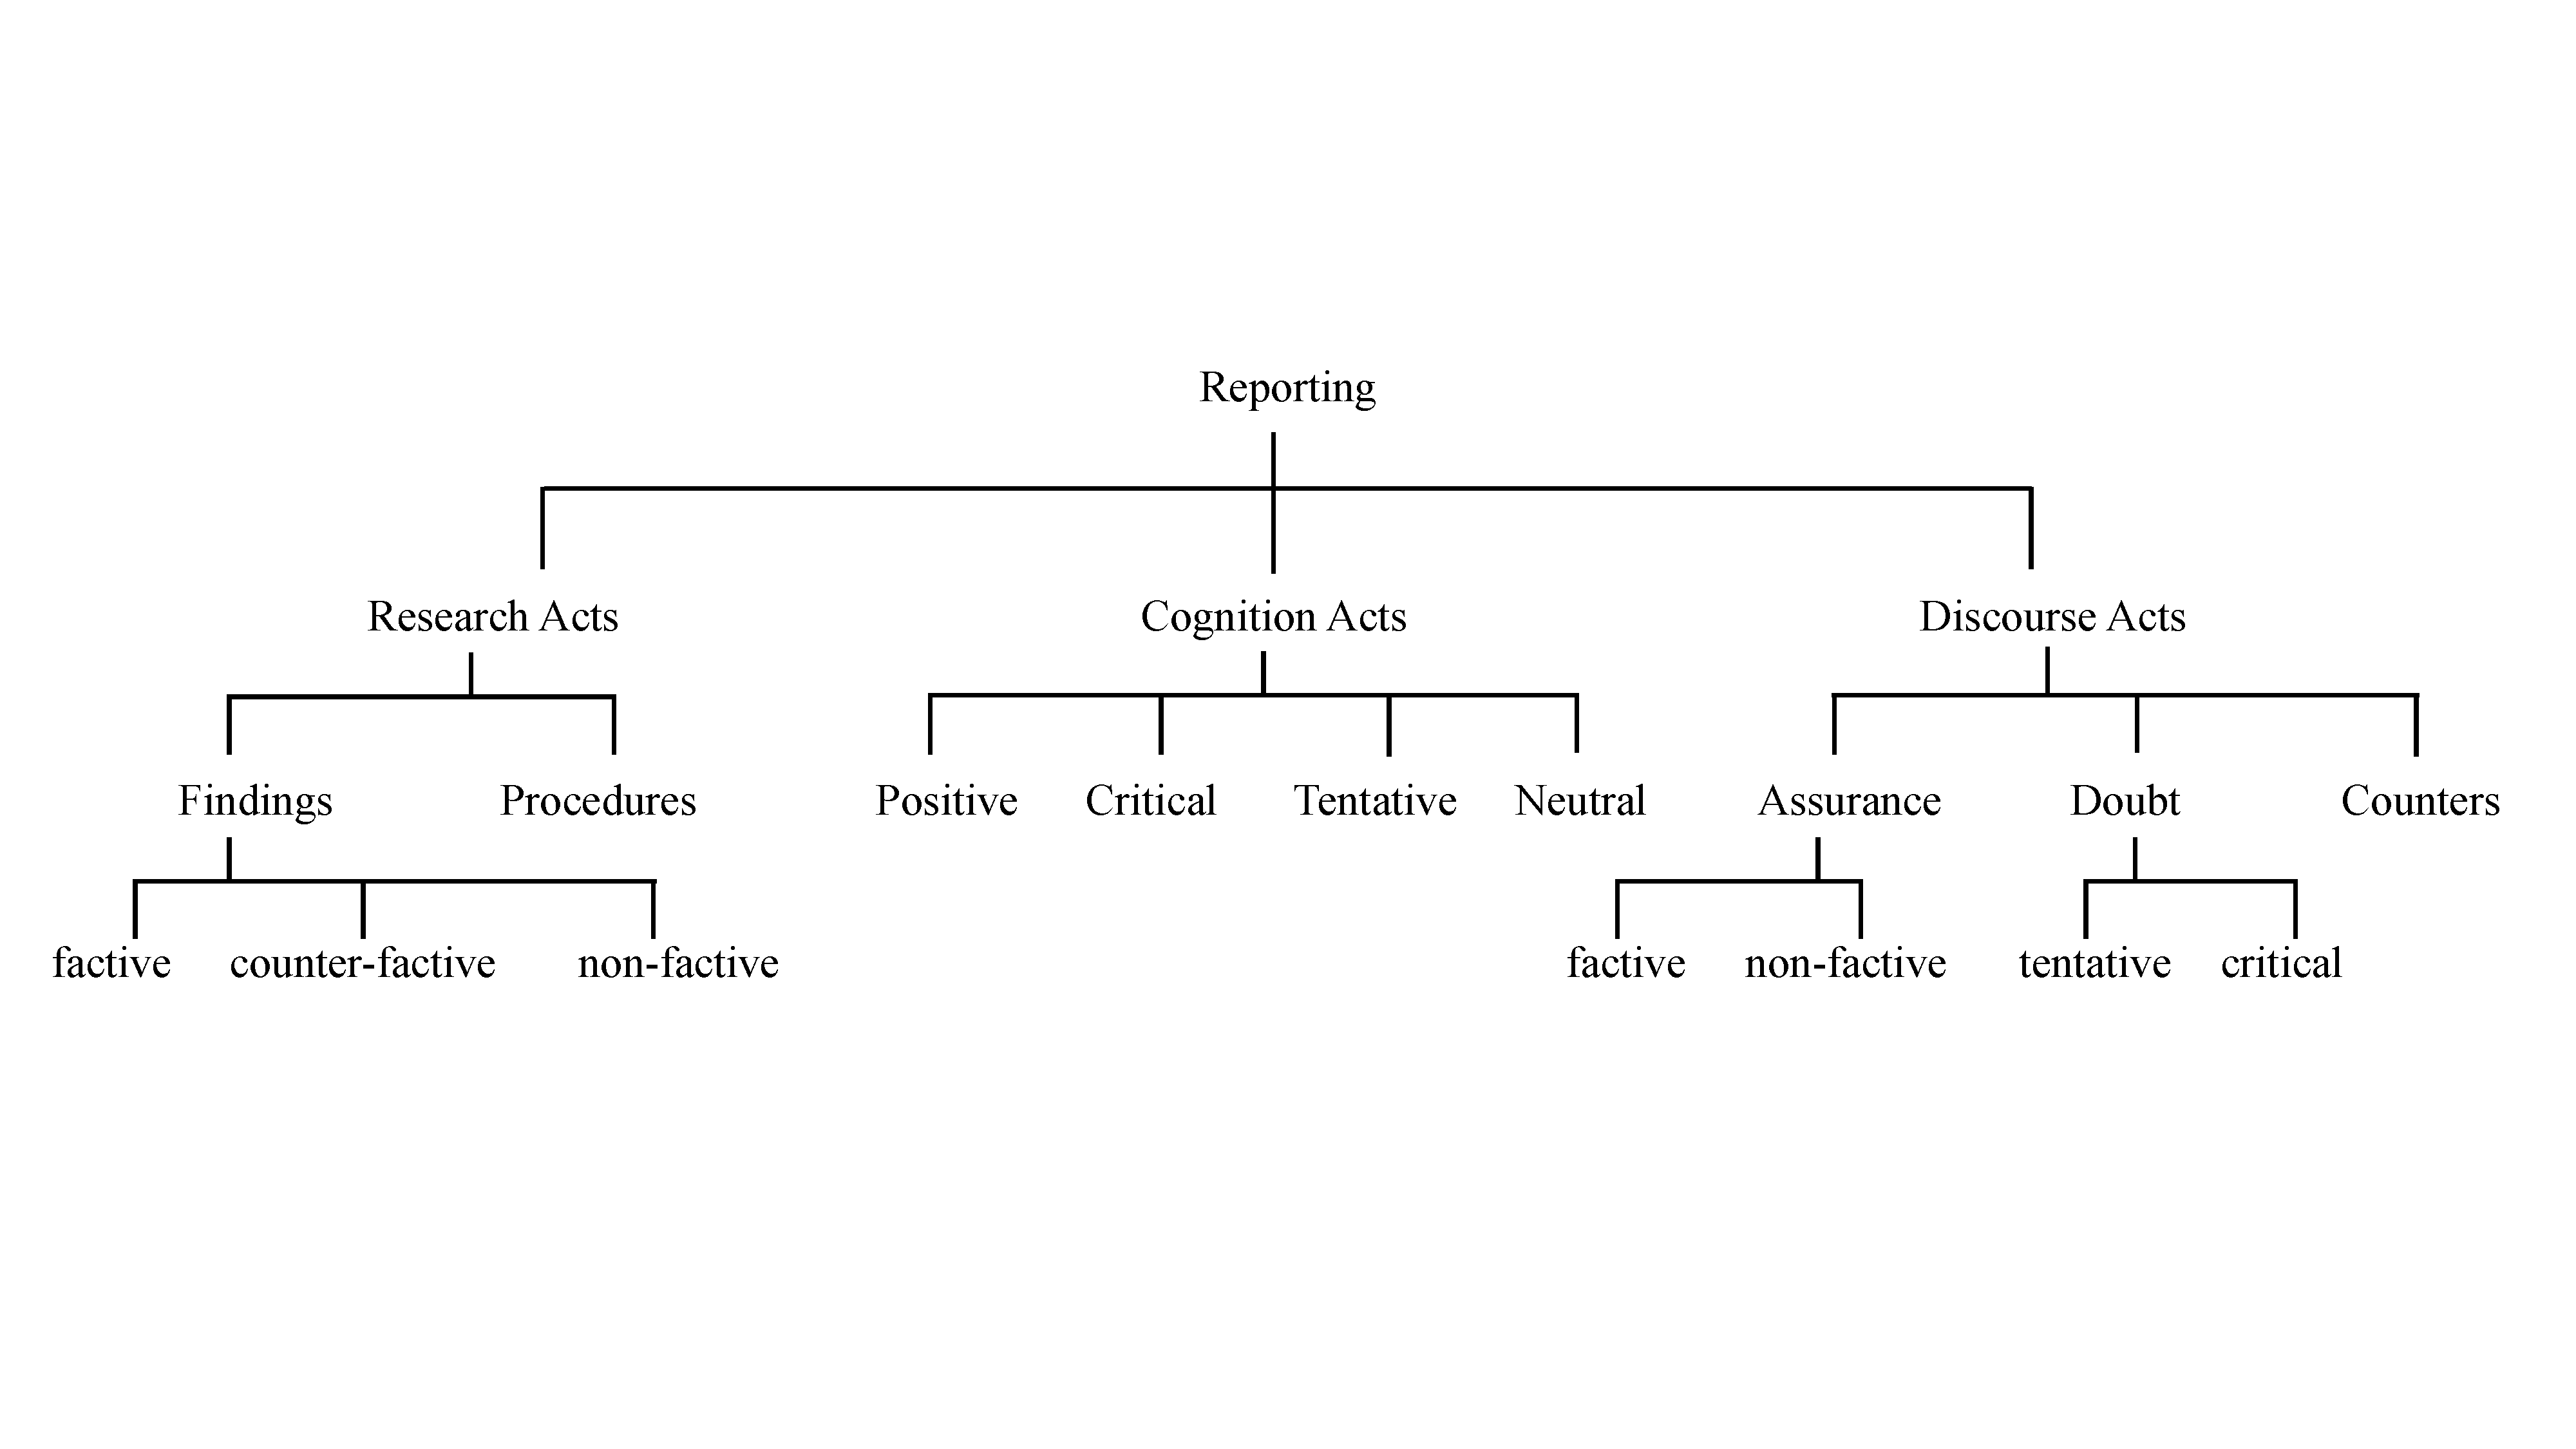
\includegraphics[width=\linewidth]{taxonomy}
    \caption[Hyland’s (2002) taxonomy of reporting verbs]{Hyland’s (2002) taxonomy of reporting verbs, reproduced from Peng’s (2019,  p.15) version.}
    \label{fig:taxonomy}
  \end{figure}

In general, several pedagogical implications on using citations pointed out by previous studies are also applicable in this study. For example, students should be informed of the different taxonomies of citations, i.e. how citations could be categorized into non-integral, integral (verb controlling), and integral (naming) in terms of form and what the different rhetorical functions or rhetorical moves of citations are (Kwan \& Chan, 2014; Mansourizadeh \& Ahmad, 2011). In the case of this study, teachers may instruct students that citations of type statement of use are often used when stating the datasets, software, and baseline models used, so that students might be less likely to make plagiarism like the case of TXT4 (missing citations for datasets and baseline models). In addition, teachers may identify research papers with proper citation use as examples and let students refer to them (Petrić \& Harwood, 2013; Ridley, 2006), or help students analyze the texts written by expert writers while highlighting on their citation use (Mansourizadeh \& Ahmad, 2011).


%%% 其它部分
\backmatter

%% 本科生要这几个索引,研究生不要。选择性留下。
% 插图索引
\listoffigures
% 表格索引
\listoftables


%% 参考文献
% 只能选择一种参考文献格式
%\bibliographystyle{thuthesis-numeric}      % 顺序编码制
\bibliographystyle{apalike}  % 著者-出版年制
% \bibliographystyle{thuthesis-bachelor}     % 本科生参考文献的著录格式
\bibliography{ref/refs}


%% 致谢
% 如果使用声明扫描页,将可选参数指定为扫描后的 PDF 文件名,例如:
% \begin{acknowledgement}[scan-statement.pdf]
\begin{acknowledgement}
  I would like to sincerely give my deep gratitude to Professor YAN Yi for her generous, professional, timely, patient, and meticulous help and instructions on my research and my thesis writing. Never before in my years at Tsinghua University had anyone offered word-by-word reviews or comprehensive advice covering both general directions and minute details like Professor YAN did. Thank you, professor.

  In my course of writing the thesis, my friend LIU Qipeng kindly accepted to take the tedious job to be my proofreader, and identified various mistakes that I might otherwise have ignored.

  The courses offered by the English Language and Literature second-degree program laid my foundation for the completion of the thesis. To my fellow classmates of the class of 2019 from the Department of Foreign Languages and Literatures and the second-degree program: it was really a fabulous and fantastic experience working with all of you. Thank you all for the countless but unique and unforgettable memories you have offered me.
\end{acknowledgement}


%% 附录
\begin{appendix}

\end{appendix}

%% 个人简历

%% 本科生进行格式审查是需要下面这个表格,答辩可能不需要。选择性留下。
% 综合论文训练记录表
\includepdf[pages=-]{scan-record.pdf}
\end{document}
